\documentclass[conference]{IEEEtran}

\usepackage[T1]{fontenc}
\usepackage[utf8]{inputenc}
\usepackage{amsmath}
\usepackage{booktabs}
\usepackage{graphicx}
\usepackage{tikz}
\usepackage{url}
\usetikzlibrary{arrows.meta, positioning}

\title{A Remote-Sensing-Enabled Landslide Monitoring and 3D Digital Twin for Tirumala Hills, India: A Verified Research Prototype}

\author{
\IEEEauthorblockN{Author Name(s)}
\IEEEauthorblockA{
\textit{Department / Institution}\\
City, State, India\\
email address(es)}
}

\begin{document}
\maketitle

\begin{abstract}
Landslide monitoring in hilly terrain requires spatially aligned observations,
data-quality controls, and clear communication of uncertainty. This paper
presents an updated implementation of a remote-sensing-enabled monitoring
prototype for Tirumala Hills, Andhra Pradesh, India. The system combines
Sentinel-1 interferometric synthetic aperture radar (InSAR) products, terrain
attributes, historical map-derived landslide locations, rainfall context, a
transparent relative-evidence index, SQLite storage, and a CesiumJS 3D
visualization. A real 12-day Sentinel-1 pair acquired on 9 and 21 November 2026
was processed through ASF HyP3, quality-checked, aligned to an 80-m grid in
WGS 84 / UTM zone 44N, and integrated into the database and viewer. The aligned
69 by 110 grid yielded 5,034 cells meeting the project's valid-LOS and
coherence-at-least-0.50 criteria. The updated database and Cesium exports
contain the observation epoch, quality information, and relative line-of-sight
(LOS) layer. A weighted evidence index reports Low, Medium, and High classes,
but is explicitly not calibrated as a landslide probability. The implementation
also includes local acquisition discovery and scheduling, although repeated
unattended processing of multiple real acquisitions has not been demonstrated.
A separate 14-channel U-Net achieved a global pixel-aggregated Dice score of
0.7188 and intersection-over-union of 0.5610 on a held-out Landslide4Sense
split; these benchmark results are not validation on Tirumala ground truth.
The prototype therefore demonstrates an auditable integration and
visualization workflow, not an operational early-warning service.
\end{abstract}

\begin{IEEEkeywords}
landslide monitoring, InSAR, digital twin, Sentinel-1, CesiumJS, evidence
integration, Tirumala Hills
\end{IEEEkeywords}

\section{Introduction}
Landslides pose a recurring risk to roads, settlements, and infrastructure in
steep terrain. Remote sensing can provide repeat observations over areas that
are difficult to survey continuously, while geographic information systems
(GIS) can help organize those observations for inspection. However, an
interactive map alone does not establish that the underlying measurements are
complete, temporally comparable, or predictive.

This work updates an earlier Tirumala Hills demonstration into a
database-backed prototype that integrates terrain, radar observations,
historical inventory context, evidence explanations, and a 3D viewer. The
implementation has a verified live Sentinel-1 InSAR-to-database-to-Cesium
workflow for one acquisition pair. It also retains local monitoring and
discovery components, a relative evidence assessment, and an independent
deep-learning demonstration on public benchmark-format patches.

The paper has four contributions:
\begin{enumerate}
    \item an auditable workflow for validating and aligning one real InSAR
    pair to a common 80-m study-area grid;
    \item a transparent, missing-data-aware relative evidence index with
    explicit non-probabilistic interpretation;
    \item database and CesiumJS integration for viewing the observation epoch,
    raster layers, and cell-level evidence; and
    \item a clear separation between verified live evidence, contextual
    datasets, benchmark model results, and capabilities that remain unverified.
\end{enumerate}

\section{Study Area and System Scope}
The study area is Tirumala Hills in Tirupati District, Andhra Pradesh, India.
The project uses an analytical grid in WGS 84 / UTM zone 44N
(EPSG:32644), with 80-m cells and a 69 by 110 raster extent. This extent
contains 7,590 grid positions; it should not be interpreted as 7,590
independent field observations.

The system is a local research prototype. It is not designed or validated as
an operational warning service. In particular, it does not claim calibrated
probabilities, field-confirmed movement, reliable cumulative displacement,
or a validated landslide prediction model. The implementation status and
live-data results reported here reflect verification performed on
22 November 2026.

\section{Data}
\subsection{Sentinel-1 InSAR}
The live observation is the descending-orbit pair
\texttt{PAIR\_20261109\_20261121}, with acquisitions on 9 and 21 November 2026.
Sentinel-1 is a C-band SAR mission \cite{sentinel1}. The pair was processed by
ASF HyP3 using its GAMMA InSAR workflow, with 20 by
4 looks, adaptive phase filtering, and MCF phase unwrapping \cite{hyp3}.
The resulting product includes LOS displacement and coherence rasters.

The aligned rasters use EPSG:32644, an 80-m resolution, and a 69 by 110 grid.
The LOS values are relative to the pair's phase reference and are not direct
vertical or three-dimensional ground-motion measurements. The product's
vertical-displacement layer is not treated as ground truth.

\subsection{Terrain and Historical Inventory}
Elevation is derived from a local digital elevation model, with slope and
aspect used as terrain descriptors. These are aligned to the project grid
before visualization; the project documents Copernicus DEM as its elevation
source \cite{copdem}. The historical inventory contains 15 approximate
locations digitized from Geological Survey of India map material \cite{gsi}. These
locations are map-derived context rather than surveyed GPS positions; the
complete bibliographic reference for the source map must be supplied before
publication.

\subsection{Rainfall Context}
The project contains a daily GPM IMERG-derived rainfall series for
1--29 August 2026, including rolling accumulation windows \cite{imerg}.
Rainfall is used as study-area temporal context, not as a pixel-level
predictor in the current evidence score. A fresh GES DISC download was not
verified; therefore, the stored series is not described as current rainfall.

\subsection{U-Net Demonstration Data}
The separate segmentation component uses 14-channel HDF5 patches compatible
with Landslide4Sense \cite{l4s}. Each patch has an \texttt{img} array of shape
128 by 128 by 14 and is processed independently of the geospatial evidence
map. The output mask is not georeferenced and is not automatically added as a
Tirumala map layer.

\section{Methods}
\subsection{Processing and Integration Workflow}
The workflow begins with Sentinel-1 product discovery and pair management.
The verified pair product is downloaded from HyP3, checked for archive
integrity, and inspected for coordinate reference system, resolution, valid
values, and NoData handling. LOS and coherence are then aligned to the
Tirumala analytical grid. Cells with missing LOS or coherence below 0.50 are
not counted as quality-screened observations; missing values are preserved
rather than replaced with zero.

The validated observation is stored in SQLite with acquisition dates,
processing status, raster paths, and quality information. Export routines
produce the Cesium layer manifest, spatial lookup, temporal registry, image
texture, and terrain model assets. A local scheduler and metadata-discovery
workflow are implemented, but only one complete real HyP3 observation cycle
has been verified.

\begin{figure*}[t]
\centering
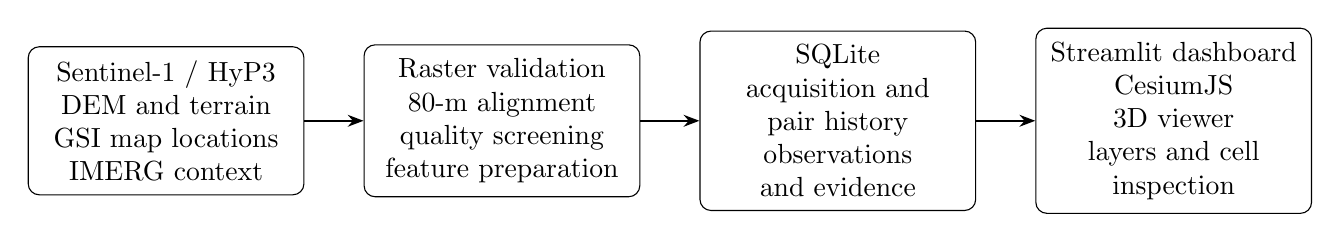
\begin{tikzpicture}[
  block/.style={draw, rounded corners, align=center, minimum height=1.35cm,
                text width=3.15cm, inner sep=5pt},
  flow/.style={-{Stealth[length=2mm]}, thick},
  node distance=0.75cm
]
\node[block] (data) {Sentinel-1 / HyP3\\DEM and terrain\\GSI map locations\\IMERG context};
\node[block, right=of data] (process) {Raster validation\\80-m alignment\\quality screening\\feature preparation};
\node[block, right=of process] (store) {SQLite\\acquisition and pair history\\observations and evidence};
\node[block, right=of store] (view) {Streamlit dashboard\\CesiumJS 3D viewer\\layers and cell inspection};
\draw[flow] (data) -- (process);
\draw[flow] (process) -- (store);
\draw[flow] (store) -- (view);
\end{tikzpicture}
\caption{Implemented data flow. The rainfall series and U-Net patch workflow are contextual or separate products; they are not treated as pixel-level live InSAR evidence.}
\label{fig:architecture}
\end{figure*}

\subsection{InSAR Quality Screening}
The project applies a coherence threshold of 0.50 as a quality-screening
rule. This is an implementation threshold, not a universal physical boundary.
The valid-cell count is the intersection of finite LOS and coherence values
with coherence at or above the threshold:
\begin{equation}
N_{\mathrm{valid}} =
\sum_{i=1}^{N}
\mathbf{1}\left[
\operatorname{finite}(d_i)
\land \operatorname{finite}(\gamma_i)
\land \gamma_i \geq 0.50
\right],
\label{eq:quality}
\end{equation}
where $d_i$ is relative LOS displacement and $\gamma_i$ is coherence. This
screen identifies cells retained for inspection; it does not independently
confirm slope movement or landslide activity.

\subsection{Relative Evidence Index}
The evidence index combines four components: slope (weight 0.40), terrain
(0.25), InSAR (0.20), and temporal evidence (0.15). The slope component is
ranked relative to the current study-area observations. The other components
are encoded as evidence indicators. For cell $i$, let $A_i$ denote the
components available for that cell, $x_{ik}$ their component values on a
0--100 scale, and $w_k$ their configured weights. The score is
\begin{equation}
S_i =
\frac{\sum_{k \in A_i} w_k x_{ik}}
     {\sum_{k \in A_i} w_k}.
\label{eq:score}
\end{equation}
If no component is available, no score is assigned. Missing components are
excluded rather than treated as zero. Evidence coverage is the available
weight divided by the total configured weight. Categories are Low
($S_i < 33.3333$), Medium ($33.3333 \leq S_i < 66.6667$), and High
($S_i \geq 66.6667$). These categories are relative evidence classes, not
calibrated probabilities or hazard forecasts.

Rainfall is intentionally not included as a cell-level score component
because the available series is study-area-level context. The dashboard's
rule-based agent and alert logic explain evidence and suggest review; they do
not constitute a separately trained predictive model.

\subsection{U-Net Segmentation and Evaluation}
The project implements a U-Net with 14 input channels and one output channel
\cite{unet}. HDF5 inputs are transformed from height--width--channel to
channel--height--width format. The sigmoid output is thresholded at 0.50 to
produce a binary mask. The trained checkpoint is evaluated using an 80/20
split with random state 42 on the local Landslide4Sense training pool. The
reported held-out set contains 760 labeled patches.

Pixel-aggregated overlap metrics are calculated from the total intersection
and union over the held-out pixels. Separately, the project also reports the
mean of batch-level overlap metrics. These aggregation schemes yield
different values and are therefore reported distinctly.

\section{Implementation}
The application uses Python for ingestion, raster processing, evidence
assessment, and the dashboard; SQLite for local persistence; and CesiumJS for
3D visualization. Raster layers are aligned in EPSG:32644 and displayed in the
web viewer with geographic coordinate transformations. The viewer includes
terrain and evidence layers, historical inventory context, observation-epoch
selection, and a spatial lookup for inspection.

Monitoring functions include Sentinel-1 metadata discovery, duplicate-aware
pair tracking, scheduled status checks, and status export. These functions
support monitoring readiness but should not be conflated with repeated
successful processing: the verified evidence at the time of assessment is
one completed live InSAR pair. Full raw Sentinel-1 scene download, fresh
IMERG retrieval, external notification delivery, and multi-pair temporal
inversion remain incomplete or unverified.

\section{Results}
\subsection{Verified Live Observation}
The live HyP3 job completed successfully and its archive integrity was
verified. The LOS and coherence rasters were aligned to the project grid.
Of 7,590 grid positions, 5,034 cells met the finite-LOS and coherence
threshold criteria. On the aligned raster, valid LOS values ranged from
$-0.111919$ m to $-0.053715$ m. These are pair-relative LOS values and are
not interpreted as vertical displacement.

The observation date was 21 November 2026. A total of 7,590 rows were
upserted for that date in the observation store: 5,034 were marked GOOD and
2,556 were missing or low quality. The row count represents grid-position
records, not 7,590 independent valid measurements.

\begin{table}[t]
\caption{Verified live-pair and evidence-index results}
\label{tab:live}
\centering
\footnotesize
\begin{tabular}{p{0.47\columnwidth}p{0.40\columnwidth}}
\toprule
\textbf{Measure} & \textbf{Reported result}\\
\midrule
Pair and interval & 9--21 Nov. 2026; 12 days\\
CRS / grid spacing & EPSG:32644 / 80 m\\
Aligned raster shape & 69 by 110\\
Grid positions & 7,590\\
Quality-screened cells & 5,034\\
Valid LOS range & $-0.111919$ to $-0.053715$ m\\
Low evidence class & 5,195 cells\\
Medium evidence class & 2,177 cells\\
High evidence class & 218 cells\\
Mean evidence score & 29.73 / 100\\
\bottomrule
\end{tabular}
\end{table}

The risk-class counts sum to the 7,590 grid-position records. Their
interpretation is limited to the implemented relative evidence index; they
are not counts of confirmed landslides. The score distribution is generated
from the available evidence components, with missing components excluded.

\subsection{Benchmark Segmentation Results}
On the held-out Landslide4Sense split, global pixel-aggregated Dice was 0.7188
and IoU was 0.5610. Precision and recall were 0.6921 and 0.7477,
respectively. Averaging the 190 batch-level overlap scores instead yielded
Dice 0.6561 and IoU 0.5101. The aggregation difference is material. Neither
metric measures Tirumala-specific performance, and the patch demonstration
does not provide georeferenced local predictions.

\begin{table}[t]
\caption{Held-out U-Net metrics on Landslide4Sense-format data}
\label{tab:unet}
\centering
\footnotesize
\begin{tabular}{lcc}
\toprule
\textbf{Aggregation} & \textbf{Dice} & \textbf{IoU}\\
\midrule
Global pixel aggregation & 0.7188 & 0.5610\\
Mean of 190 batch scores & 0.6561 & 0.5101\\
\bottomrule
\end{tabular}
\end{table}

\section{Discussion}
The principal result is an end-to-end integration of one real InSAR
observation with local persistence and 3D geospatial visualization. Quality
screening, retained NoData, and explicit LOS labeling reduce the risk of
interpreting missing or low-coherence measurements as zero movement.
The database and viewer also provide a framework for adding future
observations without presenting an unverified temporal trend.

The current temporal network is insufficient for reliable cumulative
displacement or velocity estimation. Only one quality-valid pair is verified,
and pair-specific phase references are not established as a common reference
across multiple epochs. Consequently, the November pair supports a
pair-relative LOS observation only. The older August pair records are not
used here to claim a continuous deformation time series.

The relative evidence index is useful for organizing indicators and
explaining which factors are present. Its weights and thresholds have not
been fitted to a local landslide inventory, calibrated against observed
outcomes, or independently validated. Likewise, approximate GSI map points
provide historical context but cannot serve as precise ground truth. The
Landslide4Sense benchmark provides a separate software/model check, not
evidence of local model validity.

\section{Limitations and Future Work}
This implementation has the following limitations:
\begin{itemize}
    \item only one live InSAR processing cycle is verified; repeated
    unattended processing across multiple real acquisitions is not proven;
    \item LOS is relative to the HyP3 phase reference and is not vertical or
    three-dimensional ground truth;
    \item the available valid-pair network does not support a reliable
    cumulative displacement or velocity estimate;
    \item fresh GPM IMERG retrieval was blocked, and stored rainfall is
    historical study-area context;
    \item historical GSI locations are approximate map-derived coordinates,
    and their exact source citation must be completed;
    \item the U-Net has not been validated using Tirumala-specific labeled
    observations, and its patch masks are not georeferenced; and
    \item the evidence index is not a calibrated probability or operational
    warning system.
\end{itemize}

Future work should prioritize consistent phase referencing and additional
quality-valid acquisitions, independent field/GNSS observations, a complete
and citable local landslide inventory, validated rainfall ingestion, and
evaluation of segmentation on spatially representative local labels.
Operational alerts should be considered only after independent validation,
reliability assessment, and human review procedures are established.

\section{Conclusion}
This paper describes an updated Tirumala Hills landslide-monitoring
prototype that integrates a verified real Sentinel-1 InSAR pair, aligned
terrain and radar products, SQLite records, a transparent relative evidence
index, and CesiumJS visualization. The live pair yielded 5,034
quality-screened cells on an 80-m grid. A separate U-Net benchmark evaluation
reported a global pixel-aggregated Dice score of 0.7188 and IoU of 0.5610 on
held-out Landslide4Sense data, without implying local validation.

The work demonstrates an auditable research integration, while preserving
the distinction between observation and prediction. A single verified pair,
unvalidated local risk categories, blocked fresh rainfall access, and
benchmark-only segmentation are not sufficient for operational early
warning. Further acquisition, ground validation, and calibration are required.

\begin{thebibliography}{00}

\bibitem{sentinel1}
European Space Agency, ``Sentinel-1 Mission,'' [Online]. Available:
\url{https://www.esa.int/Applications/Observing_the_Earth/Copernicus/Sentinel-1}.

\bibitem{hyp3}
Alaska Satellite Facility, ``HyP3 Documentation,'' [Online]. Available:
\url{https://hyp3-docs.asf.alaska.edu/}.

\bibitem{imerg}
NASA, ``Global Precipitation Measurement (GPM) Integrated Multi-satellitE
Retrievals for GPM (IMERG),'' [Online]. Available:
\url{https://gpm.nasa.gov/data/imerg}.

\bibitem{copdem}
Copernicus Data Space Ecosystem, ``Copernicus Digital Elevation Model
(DEM),'' [Online]. Available:
\url{https://spacedata.copernicus.eu/collections/copernicus-digital-elevation-model}.

\bibitem{unet}
O. Ronneberger, P. Fischer, and T. Brox, ``U-Net: Convolutional Networks for
Biomedical Image Segmentation,'' in \textit{Medical Image Computing and
Computer-Assisted Intervention (MICCAI)}, 2015, pp. 234--241,
doi: 10.1007/978-3-319-24574-4\_28.

\bibitem{l4s}
O. Ghorbanzadeh \textit{et al.}, ``Landslide4Sense: Reference benchmark data
and deep learning models for landslide detection,'' \textit{IEEE
Transactions on Geoscience and Remote Sensing}, vol. 60, 2022.

\bibitem{gsi}
Geological Survey of India, \textit{[Insert the exact inventory/report title,
figure number, publication year, and page used to digitize the Tirumala
locations before submission].}

\end{thebibliography}

\end{document}
